\documentclass{beamer}
\mode<presentation> 
{
	\usetheme[alternativetitlepage]{Torino}
	\usecolortheme{chameleon}
	\setbeamercovered{transparent}	
}
\usepackage{ucs}
\usepackage[utf8x]{inputenc}
\usepackage[czech]{babel}
\usepackage{palatino}
\usepackage{graphicx}
\usepackage{epstopdf}
\usepackage{color}
\usepackage[export]{adjustbox}
\usepackage{multicol}
\usepackage{hyperref}
\usepackage{subcaption}
\usepackage{caption}
\usepackage[]{algorithm2e}
\usepackage{amsmath}

\captionsetup{labelformat=empty,labelsep=none}


\definecolor{olive}{RGB}{51, 149, 48}
\definecolor{red}{RGB}{195, 2, 36}

\definecolor{gred}{RGB}{196, 66, 48}
\definecolor{glime}{RGB}{168, 189, 4}
\definecolor{ggreen}{RGB}{57,181,74}

\title{\textbf{Detekce objektů na CUDA, jejich rozpoznání a sledování}}
\author{
	\large{Pavel Macenauer} \\ 
	\tiny{xmacen02@stud.fit.vutbr.cz} \\ 
	\large{Jan Bureš} \\ 
	\tiny{xbures19@stud.fit.vutbr.cz}
}
\date{\tiny{\today}}
\institute[FIT VUTBR]
{
	\inst{}
	Fakulta Informačních Technologií \\
	Vysoké Učení Technické v Brně
}

\begin{document}

	\begin{frame}[t,plain]
	\titlepage
	\tableofcontents[currentsection]
	\vspace{-10mm}
	\center{ 
\includegraphics[height=9mm]{logo.eps} }
	\end{frame}

%% ------------- SNIMAC -------------

	\begin{frame}[t,fragile]
		\frametitle{Obsah}	
		
		\begin{itemize}
			\item Cíl práce
			\item Detekce objektů
			\item Implementace detektoru obličejů na GPU
			\item Trackování a rozpoznání obličeje
			\item Výstup a ukázka		
		\end{itemize}			
				
	\end{frame}
	

	
	%% -----------------------------
	
	\begin{frame}[t,fragile]
		\frametitle{Cíl práce}
		
		\begin{itemize}
			\item Detektor obličejů na CUDA
			\item Trackování obličejů
			\item Rozpoznání obličeje
		\end{itemize}		
		
	\end{frame}


%% ------------------------------

	\begin{frame}[t,fragile]
		\frametitle{Detekce objektů}
		
		\begin{itemize}
			\item \textbf{Waldboost} \\ Metaalgoritmus, který skládá slabé klasifikátory v jeden silný. V každém kroku kontroluje, zda-li nepřesáhl danou mez a případně skončí.
			\item slabý klasifikátor - \textbf{LBP} příznaky
		\end{itemize}	
			

	\end{frame}
	
		%% --------------------------

	\begin{frame}[t,fragile]
		\frametitle{Waldboost}					
		\centering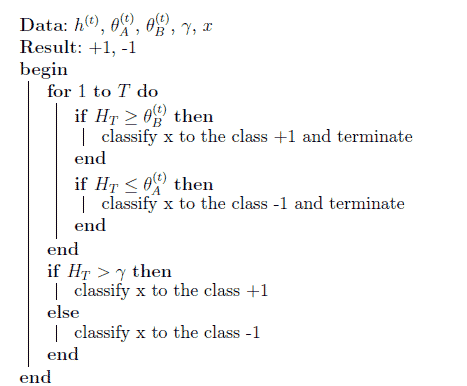
\includegraphics[width=8cm]{img/waldboost.png}
		
	
	\end{frame}
	
	%% --------------------------
	
		\begin{frame}[t,fragile]
		\frametitle{LBP příznaky}	
			
\centering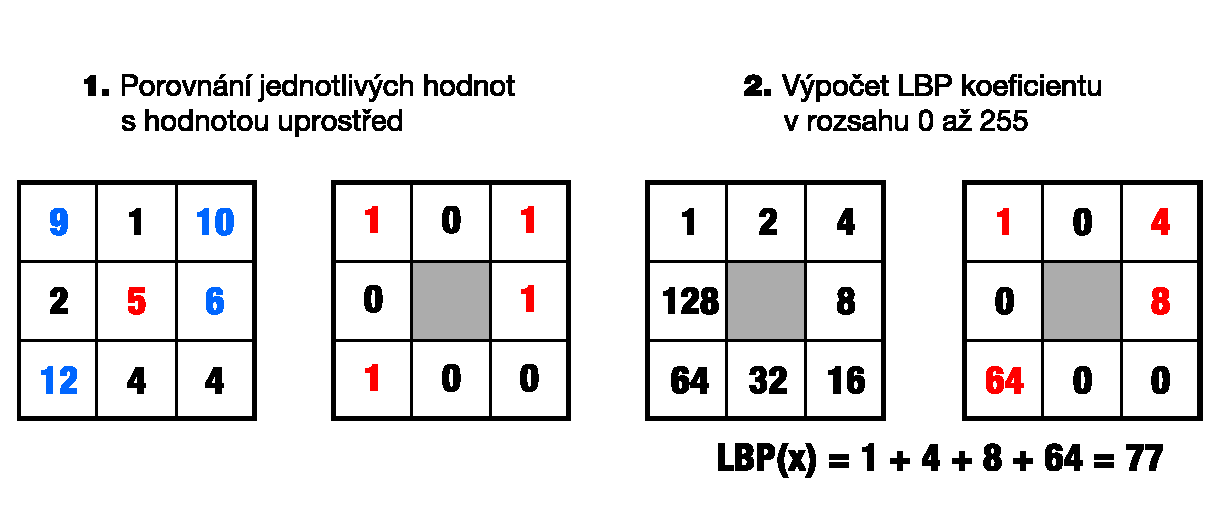
\includegraphics[width=8cm]{img/lbp.eps}

\begin{itemize}
	\item Pro každý pixel prochází 1 až N stages
	\item Pro daný stage spočte LBP = kód a z tabulky určí odezvu
	\item Ukončí výpočet, pokud odezva přesáhne mez
	\item Dojde-li nakonec stages, zkontroluje konečnou mez a rozhodne	
\end{itemize}


								
	\end{frame}		
	
	%% --------------------------
	
	\begin{frame}[t,fragile]
		\frametitle{Implementace}
		2 fáze (kernely):
		\begin{enumerate}		
	    	\item Postavení pyramidového obrazu \\
	    	Pro každý pixel původního obrazu se rozběhne vlákno a generuje N zmenšenin
			\item Detekce objektů \\
			Pro každý pixel pyramidového obrazu se rozběhne vlákno a vyhodnocuje příznaky.		
			\item Detekce je většinou nalezena na podvzorkovaném obraze - přepočítání na původní
		\end{enumerate}
		
	\end{frame}
	
	\begin{frame}[t,fragile]
		\frametitle{Pyramidový obraz}	
			
\centering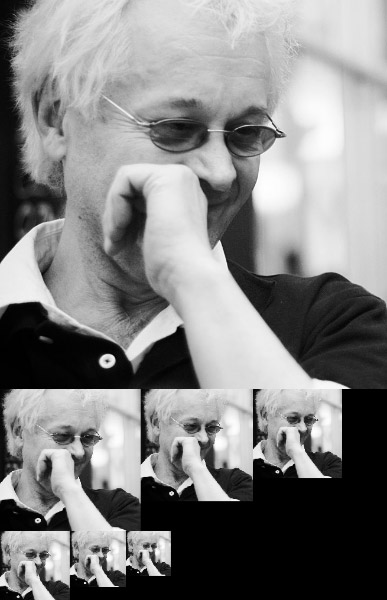
\includegraphics[width=4.5cm]{img/pyramid.jpg}

								
	\end{frame}		
	
	
		\begin{frame}[t,fragile]
		\frametitle{Uspořádání detektoru na GPU - v CUDA paměti}
		\begin{itemize}
\item \textbf{Stages} – constant memory
\item \textbf{Alphas} – texture (global) memory
\item \textbf{Původní obraz} – texture (global) memory
\item \textbf{Pyramidový obraz} – texture (global) memory
\item \textbf{Obrazové parametry} – constant memory
\end{itemize}
		
	\end{frame}
	
%% --------------------------

	\begin{frame}[t,fragile]
		\frametitle{Optimalizace}					
		
		\begin{itemize}
			\item Detektor vyexportován z XML do \verb|C++| headeru
			\item Příznaky jsou max. velikosti 2x2 \\
				  Bilineární interpolace jednotlivých LBP hodnot na HW pomocí texturovací paměti
				  \item Stages v konstantní paměti - umožňuje broadcast
				  \item Slabá podpora mipmap přímo pomocí CUDA. Pyramidový obraz? Bilineární interpolace pomocí texturovací paměti na HW
				  \item Seskládání pyramidového obrazu, aby zabíral méně prostoru
		\end{itemize}

	\end{frame}
		
		
	\begin{frame}[t,fragile]

		\vspace{30mm}
\centering
\Huge Děkujeme za pozornost.\\ Otázky?
						
		
	\end{frame}

	
\end{document} 
